%! TeX program = lualatex
\documentclass[main]{subfiles}

\begin{document}

\title[AutoML: BO]{Basic BO Loop and Surrogate Modeling}
\subtitle{Initial Design, Surrogate Modeling, and Iterative Loop}
\author[Bernd Bischl]{Bernd Bischl}
\date{}

\titlebackground*{images/AutoML_HPO_2_2}

%\institute{}
%\date{}

    \maketitle


\begin{frame}{Optimization via Surrogate Modeling}
  \begin{itemize}
    \item Want to solve  $$\conf^\ast \in \argmin_{\conf \in \pcs} \cost(\conf)$$
    \item We do not know the analytical structure of $\cost: \pcs \to \R$
    \item $\cost$ is more a computer program we can evaluate for some inputs $\conf \in \pcs$
    \item For now, we assume that those evaluations are noise-free
    \item \textbf{Idea:} Use historical data $\Dt = \{(\confI{i},  \cost(\confI{i}))\}_{i = 1, \ldots, t}$
    to learn as much about $\cost$ as we can, to intelligently plan design points sequentially
  \end{itemize}
  \vfill
    \begin{center}
        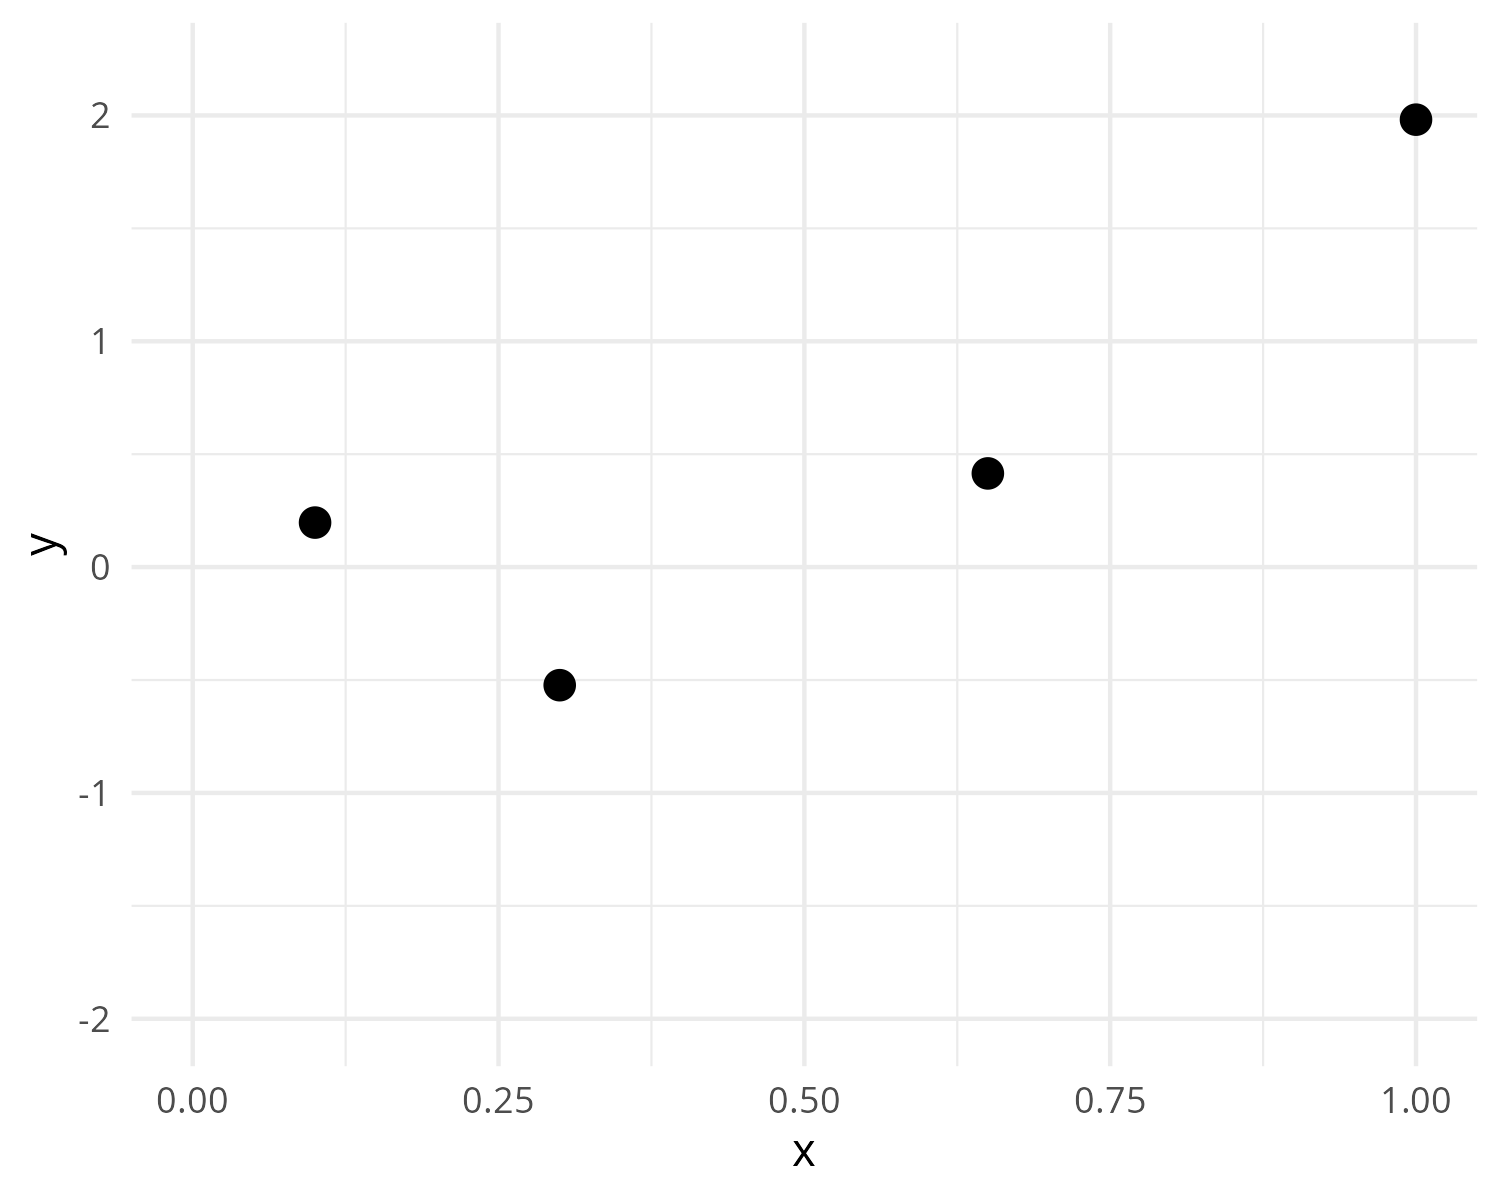
\includegraphics[width=.2\textwidth]{images/loop_1.png}
    \end{center}
\end{frame}

%----------------------------------------------------------------------

\begin{frame}{Initial Design}
    \begin{itemize}
        \item Should cover / explore the input space sufficiently:
            \begin{itemize}
                \item Random design
                \item Latin hypercube sampling
                \item Sobol sampling
            \end{itemize}
        \item Type of design usually does not have the largest effect
        \item A more important choice is the \textbf{size} of the initial design
            \begin{itemize}
                \item Should neither be too small (bad initial fit) nor too large (spending too much budget without ``intelligent'' optimization)
                \item Rule of thumb: $4d$
            \end{itemize}
    \end{itemize}
\end{frame}

%----------------------------------------------------------------------

\begin{frame}{Latin Hypercube Sampling}
    \begin{columns}
        \column{.5\textwidth}
        \begin{itemize}
            \item LHS partitions the search space into bins of equal probability
            \item Goal: attain a more even distribution of sample points than random sampling
            \item Allow at most one sample per bin; exactly one sample per row and column
        \end{itemize}
        \column{.5\textwidth}
        \begin{center}
            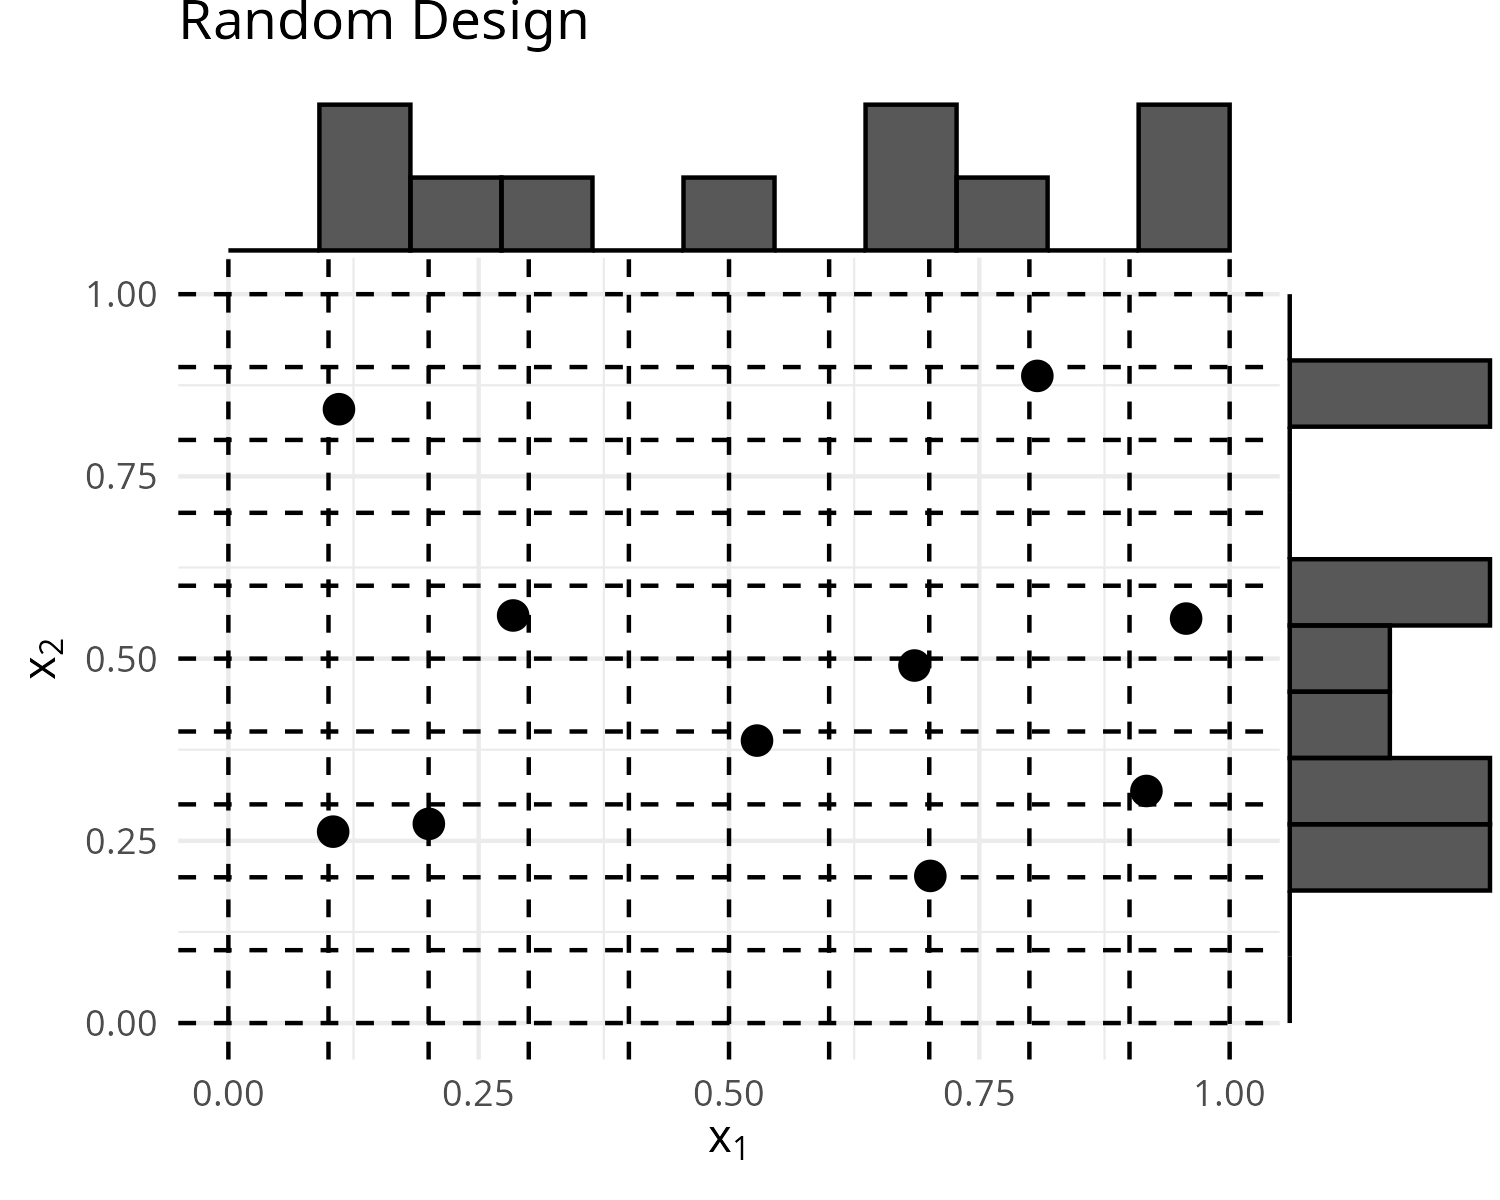
\includegraphics[width=.75\textwidth]{images/init_0.png}\\
            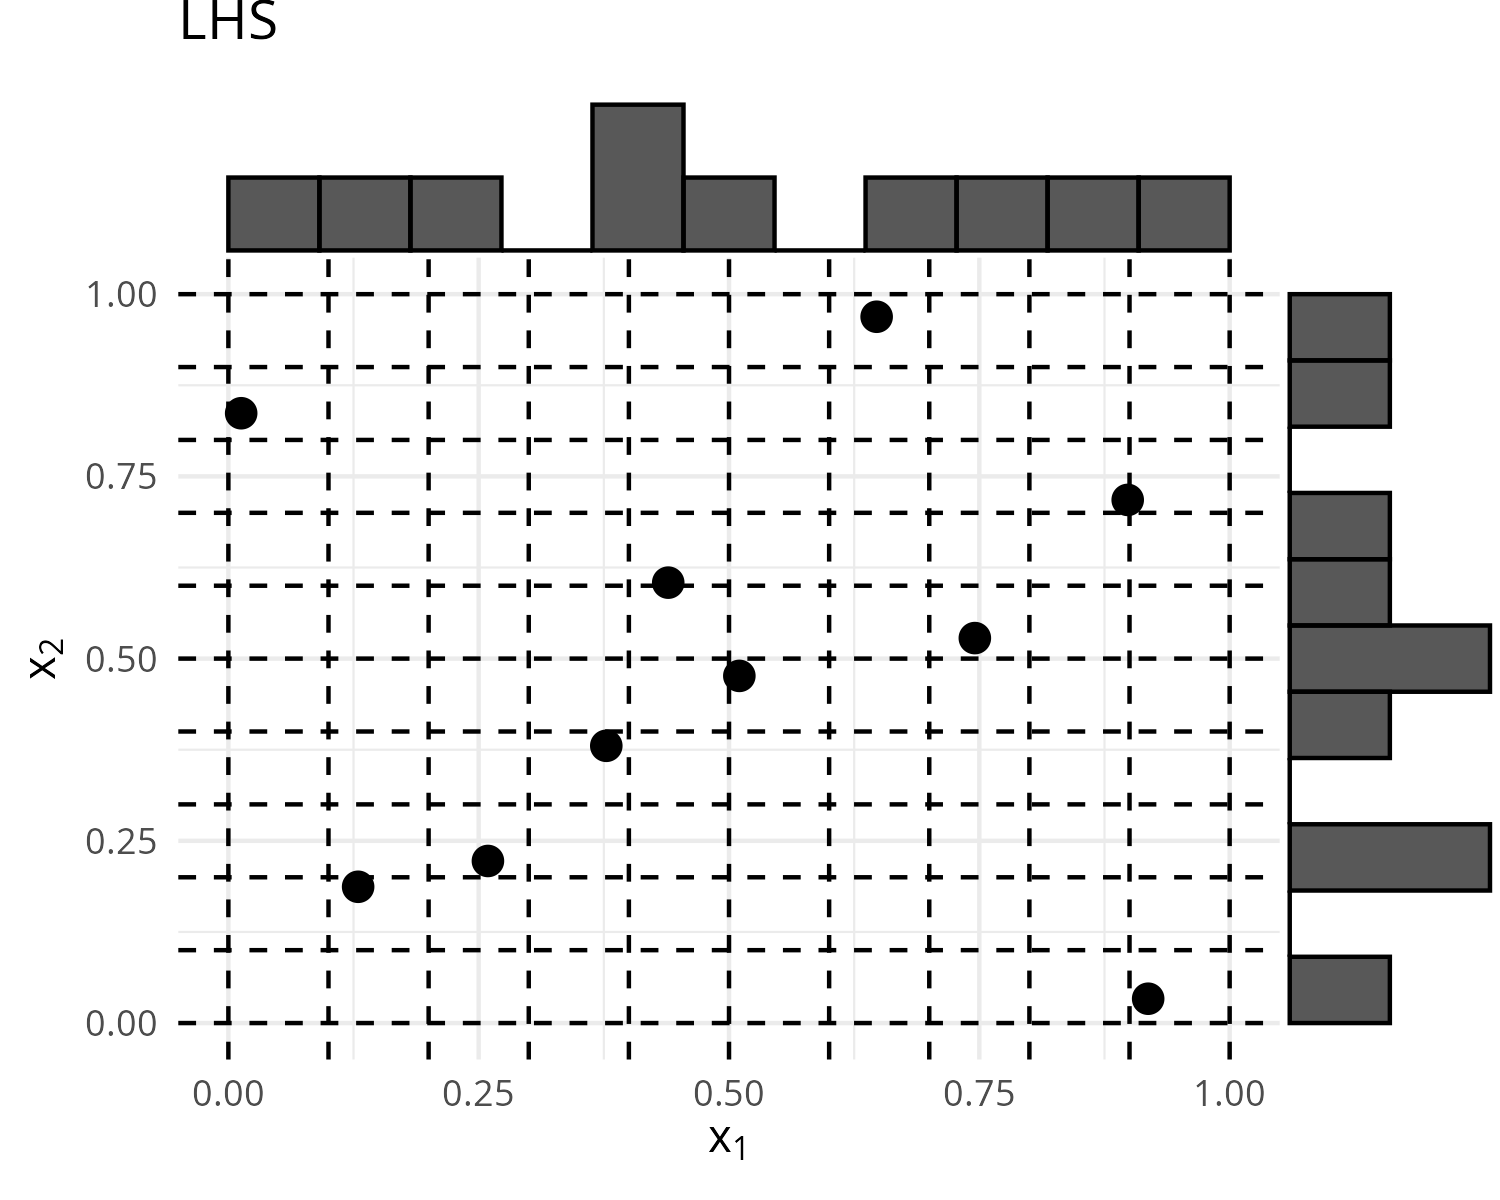
\includegraphics[width=.75\textwidth]{images/init_1.png}\\
            \footnotesize Marginal histograms: RS vs.\ LHS
        \end{center}
    \end{columns}
\end{frame}

%----------------------------------------------------------------------

\begin{frame}{Latin Hypercube Sampling}
    Actual sampling of points, e.g.\ constructed via \textbf{Maximin}:
    \begin{itemize}
        \item The minimum distance between any two points in $\D$ is $2q = \min_{\conf \in \D, \conf' \in \D} \rho(\conf, \conf')$ ($\rho$ any metric, e.g.\ Euclidean distance)
        \item $q$ is the packing radius: the radius of the largest ball that can be placed around every design point such that no two balls overlap
        \item Goal: find $\D$ that maximizes $2q$: $\max_{\D} \min_{\conf \in \D, \conf' \in \D} \rho(\conf, \conf')$
        \item Ensures that the design points in $\D$ are as far apart from each other as possible
    \end{itemize}
\end{frame}

%----------------------------------------------------------------------

\begin{frame}{Surrogate Modeling}
    Running example: minimize this ``black-box''.
    \vfill
    \begin{center}
        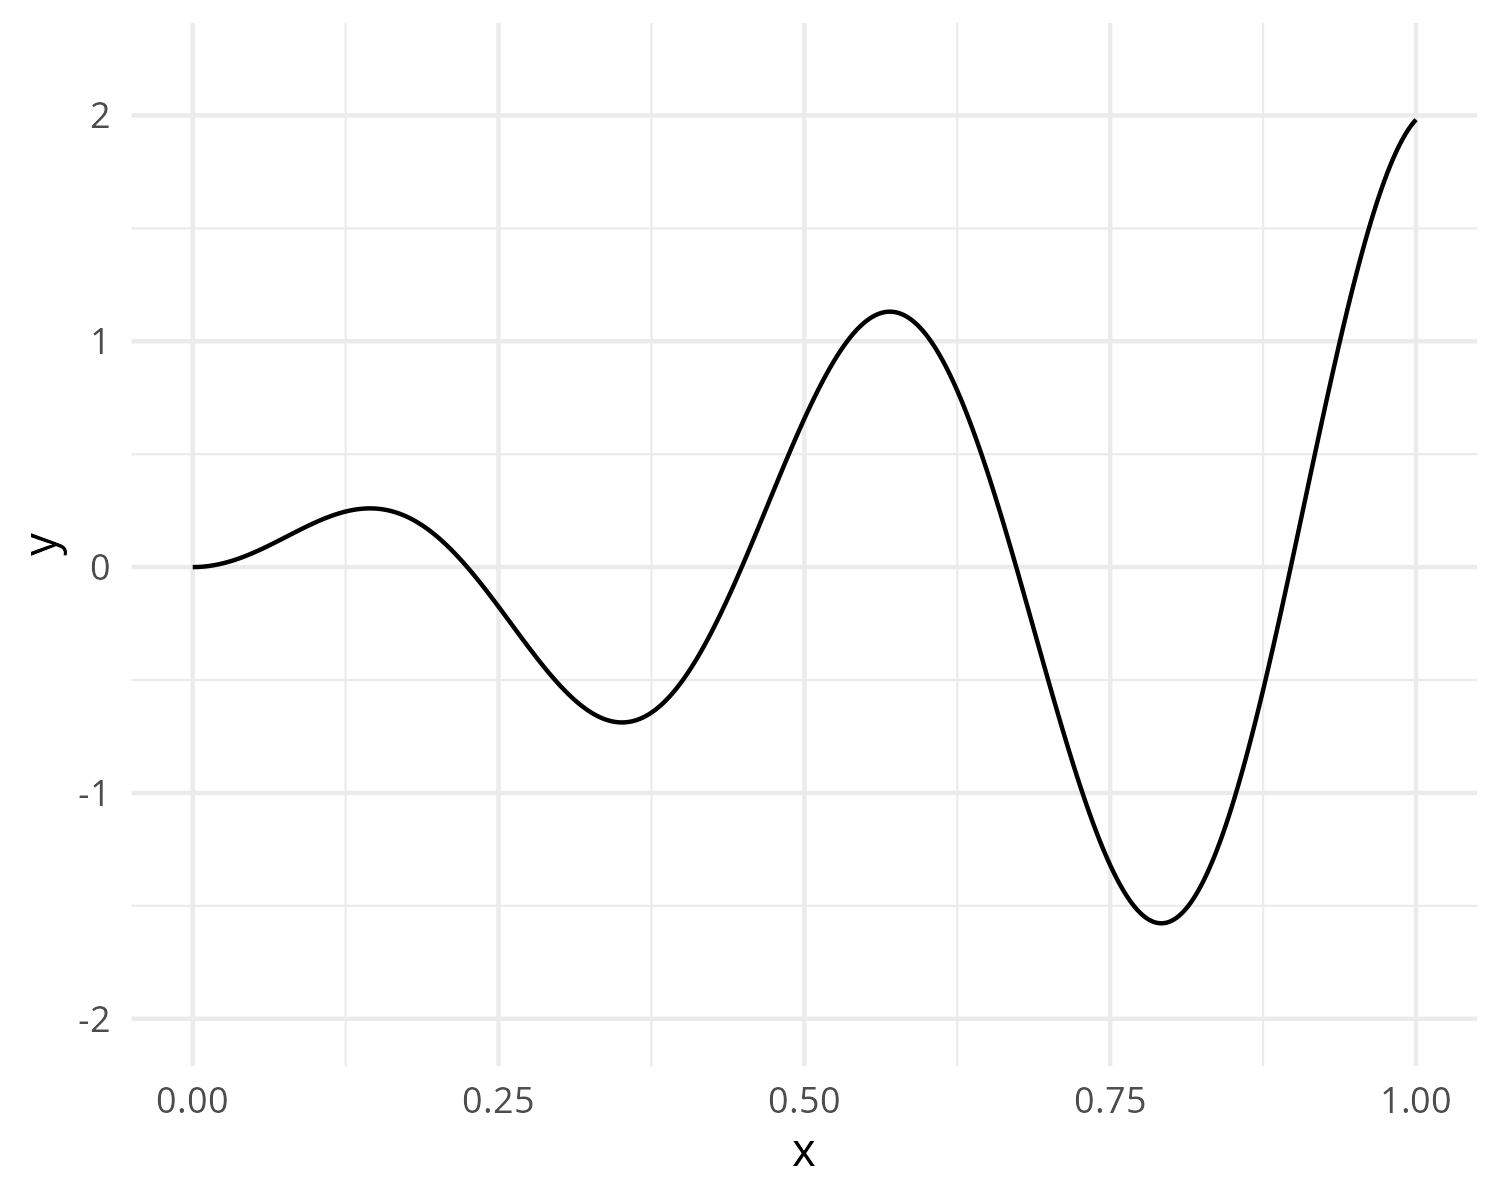
\includegraphics[width=.8\textwidth]{images/loop_0.png}
    \end{center}
\end{frame}

%----------------------------------------------------------------------

\begin{frame}{Surrogate Modeling}
    \textbf{Fit} a \textbf{regression model} $\surro: \Dt \to \R$ (blue) to extract maximum information from the design points (black) and learn properties of $\cost$.
    \vfill
    \begin{center}
        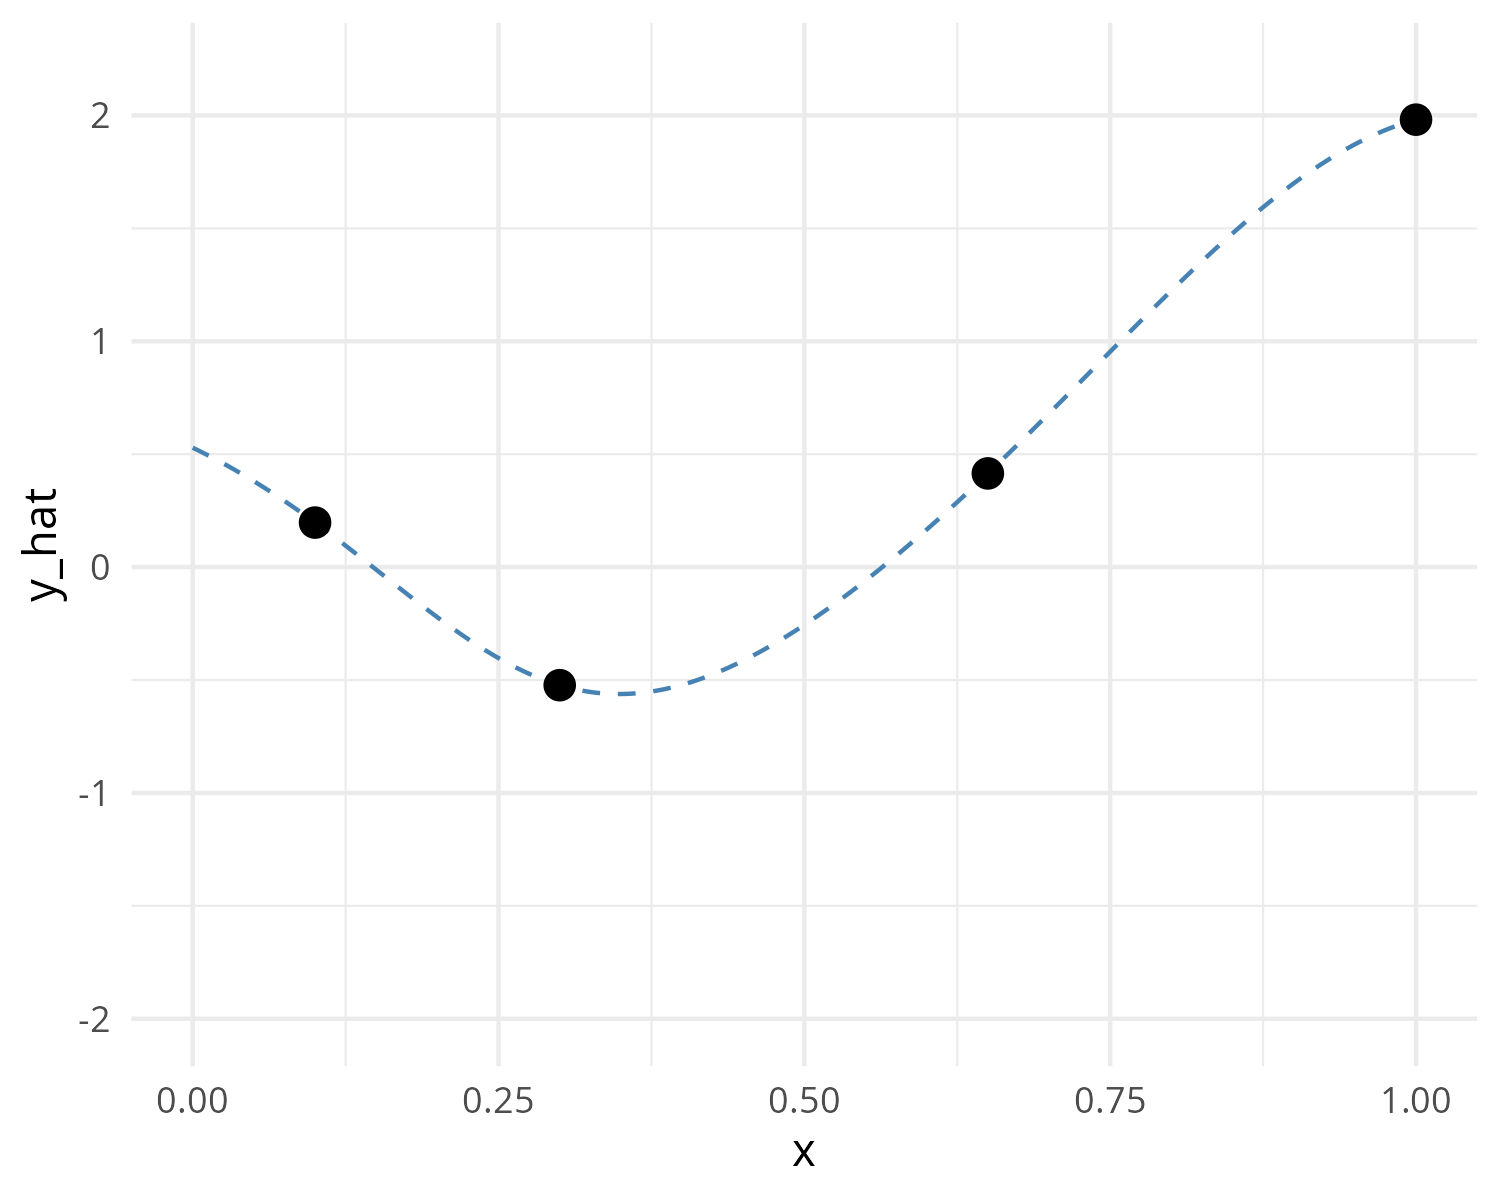
\includegraphics[width=.7\textwidth]{images/loop_2.png}
    \end{center}
    \begin{center}
        As we can evaluate $\cost$ without noise, we fit an interpolator.
    \end{center}
\end{frame}

%----------------------------------------------------------------------

\begin{frame}{Surrogate Modeling}
    Instead of the expensive $\cost$, we optimize the cheap surrogate $\surro$ (blue) to \textbf{propose} a new point (red) for evaluation.
    \vfill
    \begin{center}
        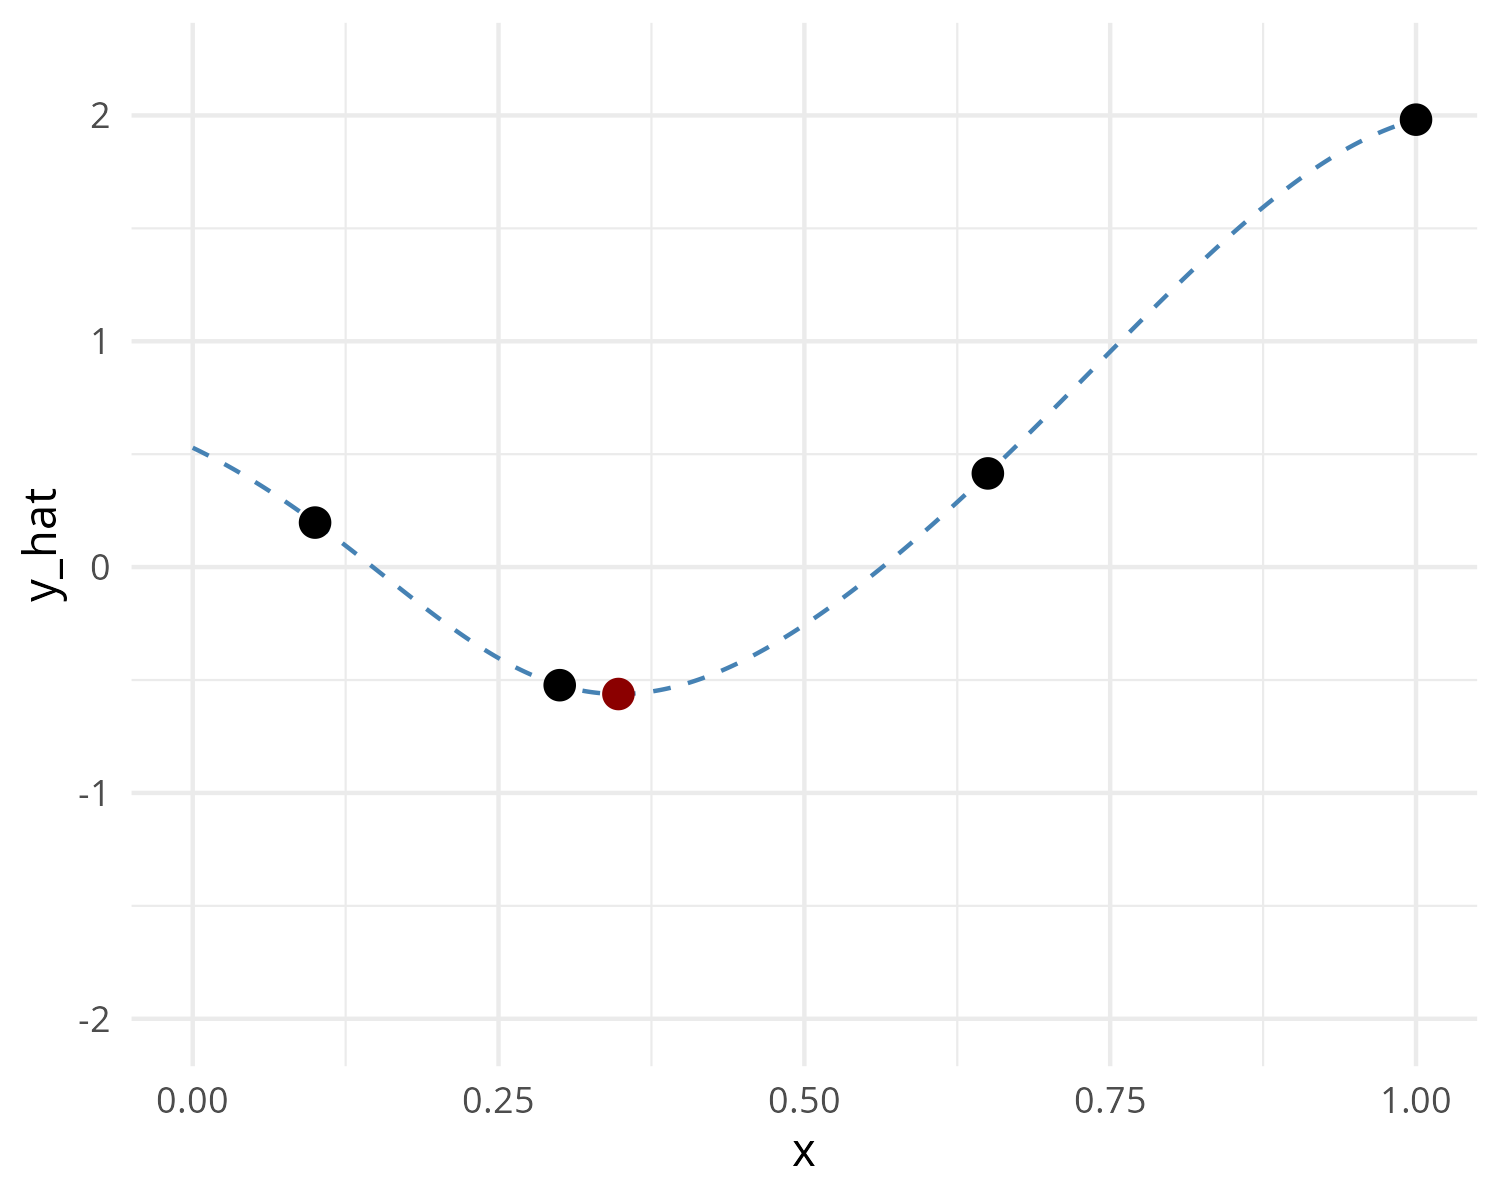
\includegraphics[width=.7\textwidth]{images/loop_3.png}
    \end{center}
\end{frame}

%----------------------------------------------------------------------

\begin{frame}{Surrogate Modeling}
    We finally evaluate the newly proposed point.
    \vfill
    \begin{center}
        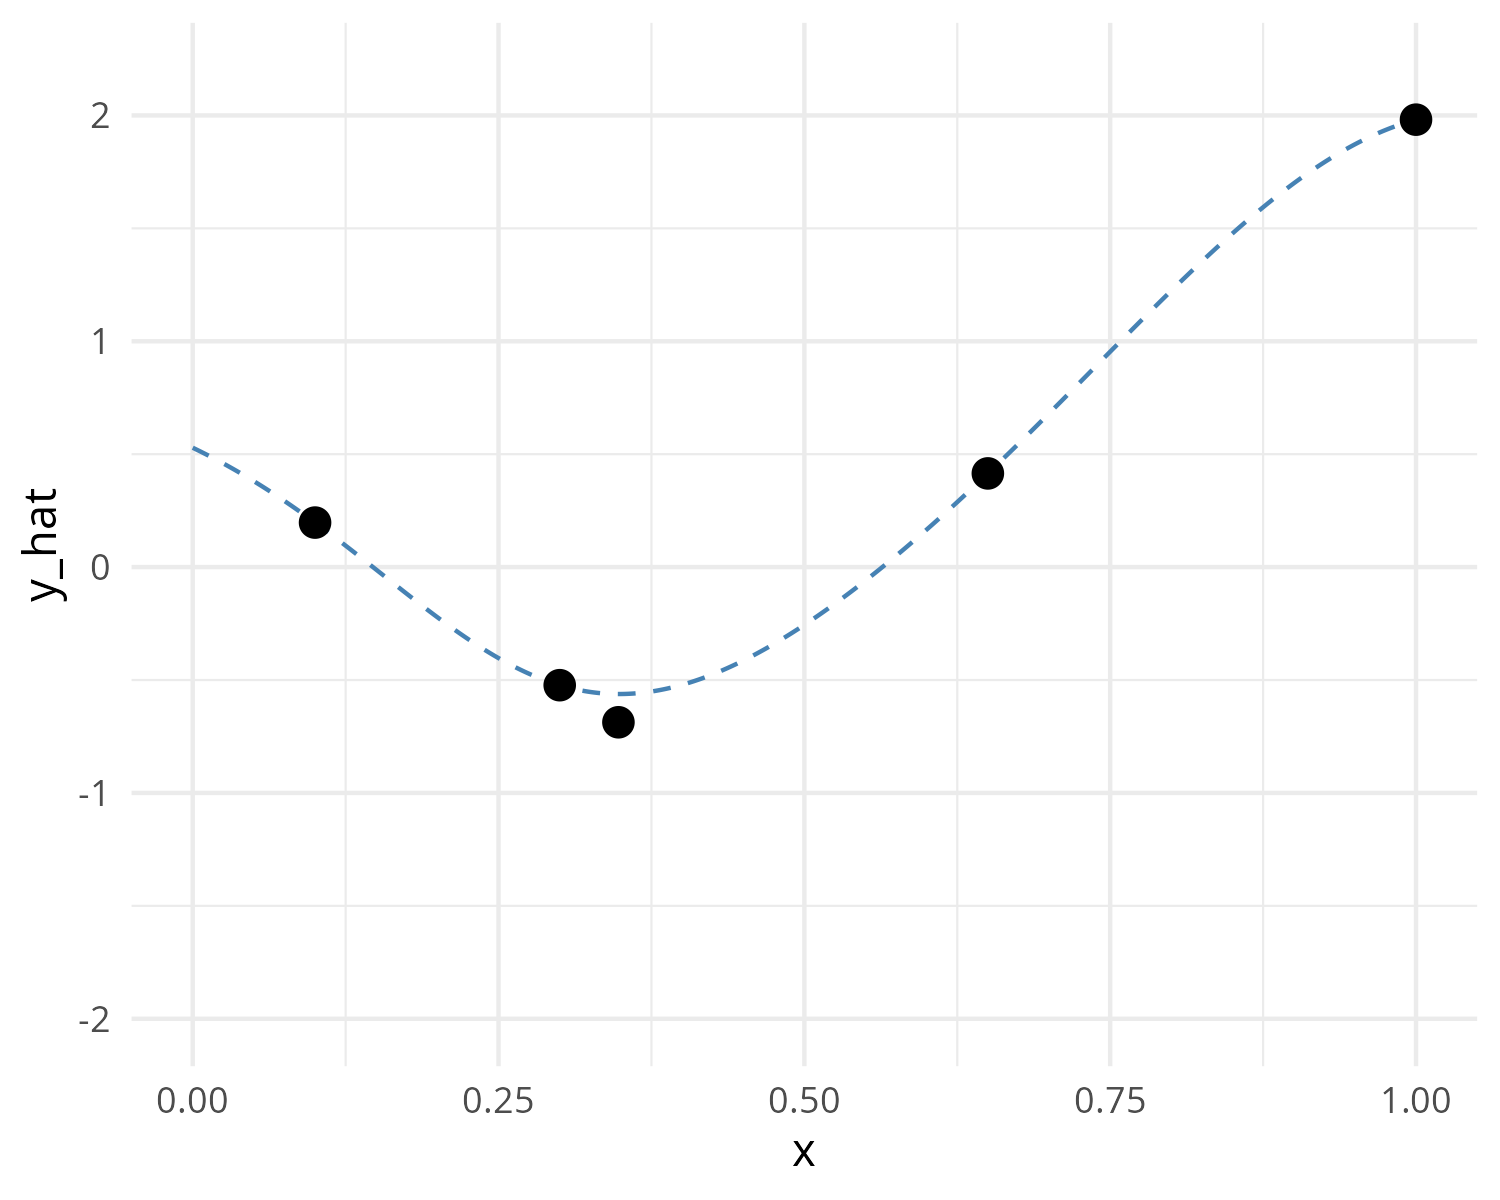
\includegraphics[width=.7\textwidth]{images/loop_4.png}
    \end{center}
\end{frame}

%----------------------------------------------------------------------

\begin{frame}{Surrogate Modeling}
    After evaluation of the new point, we \textbf{adjust} the model on the expanded dataset via (slower) refitting or a (cheaper) online update.
    \vfill
    \begin{center}
        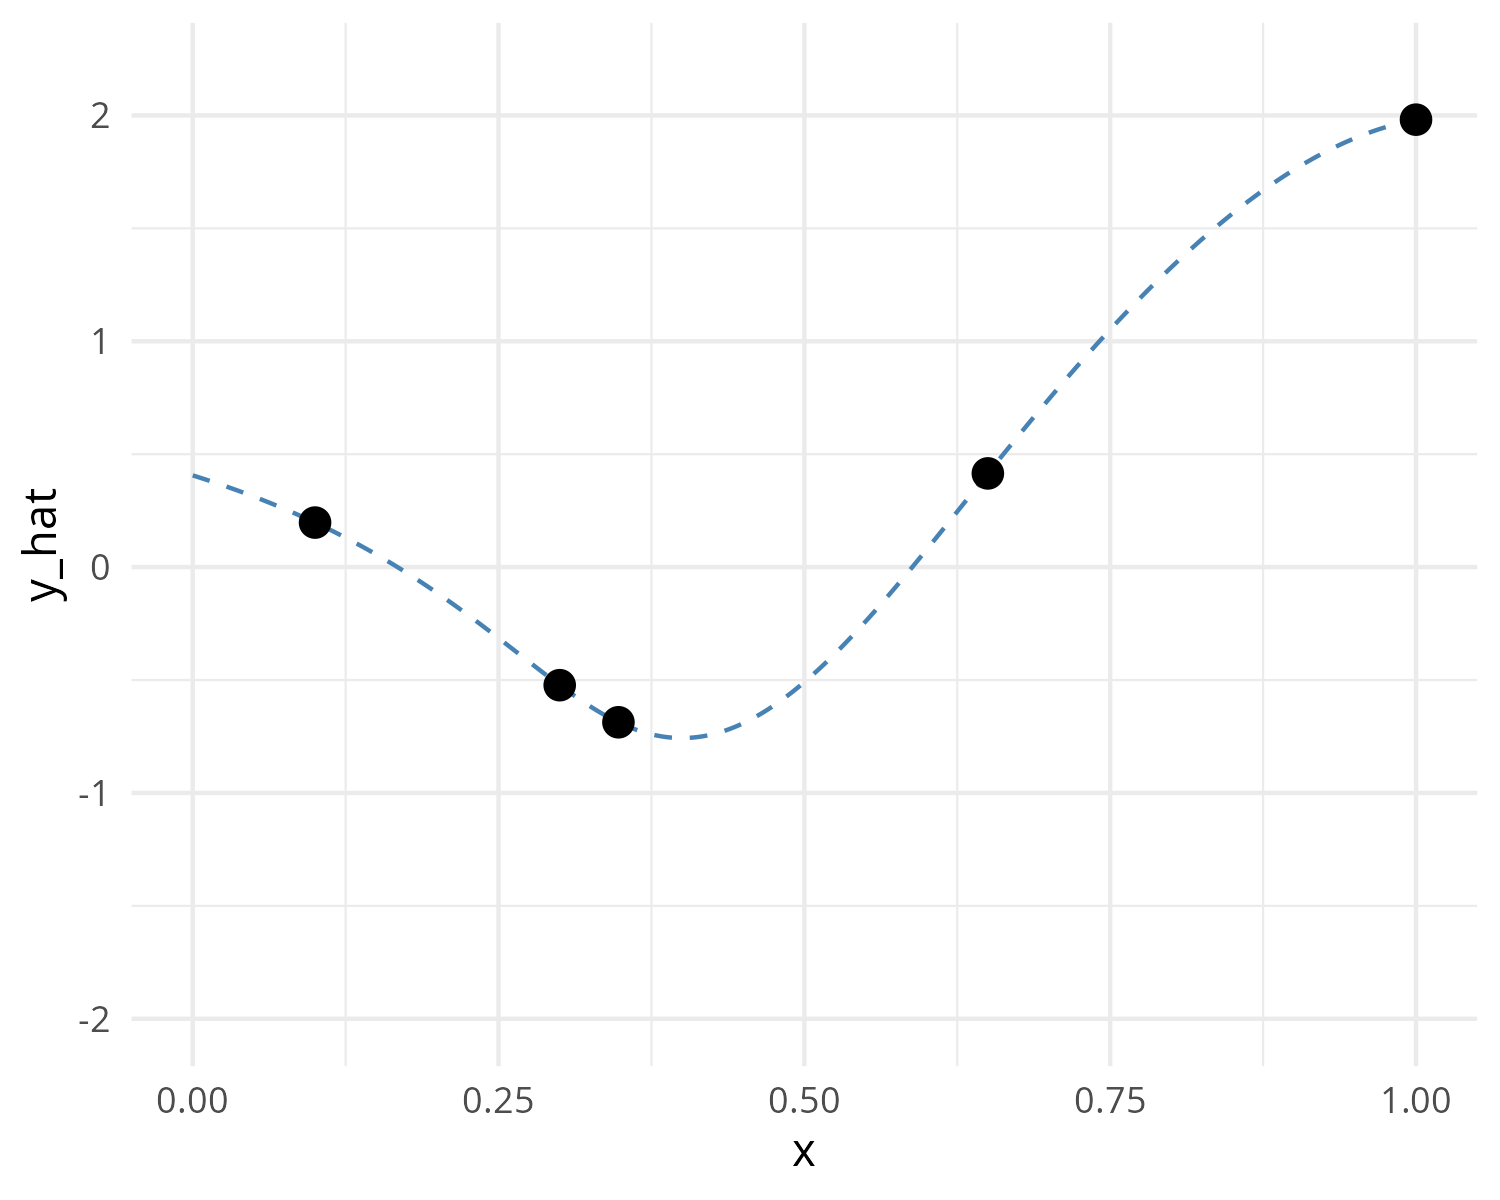
\includegraphics[width=.7\textwidth]{images/loop_5.png}
    \end{center}
\end{frame}

%----------------------------------------------------------------------

\begin{frame}{Surrogate Modeling}
    We again obtain a new candidate point (red) by optimizing the cheap surrogate model function (blue)\ldots
    \vfill
    \begin{center}
        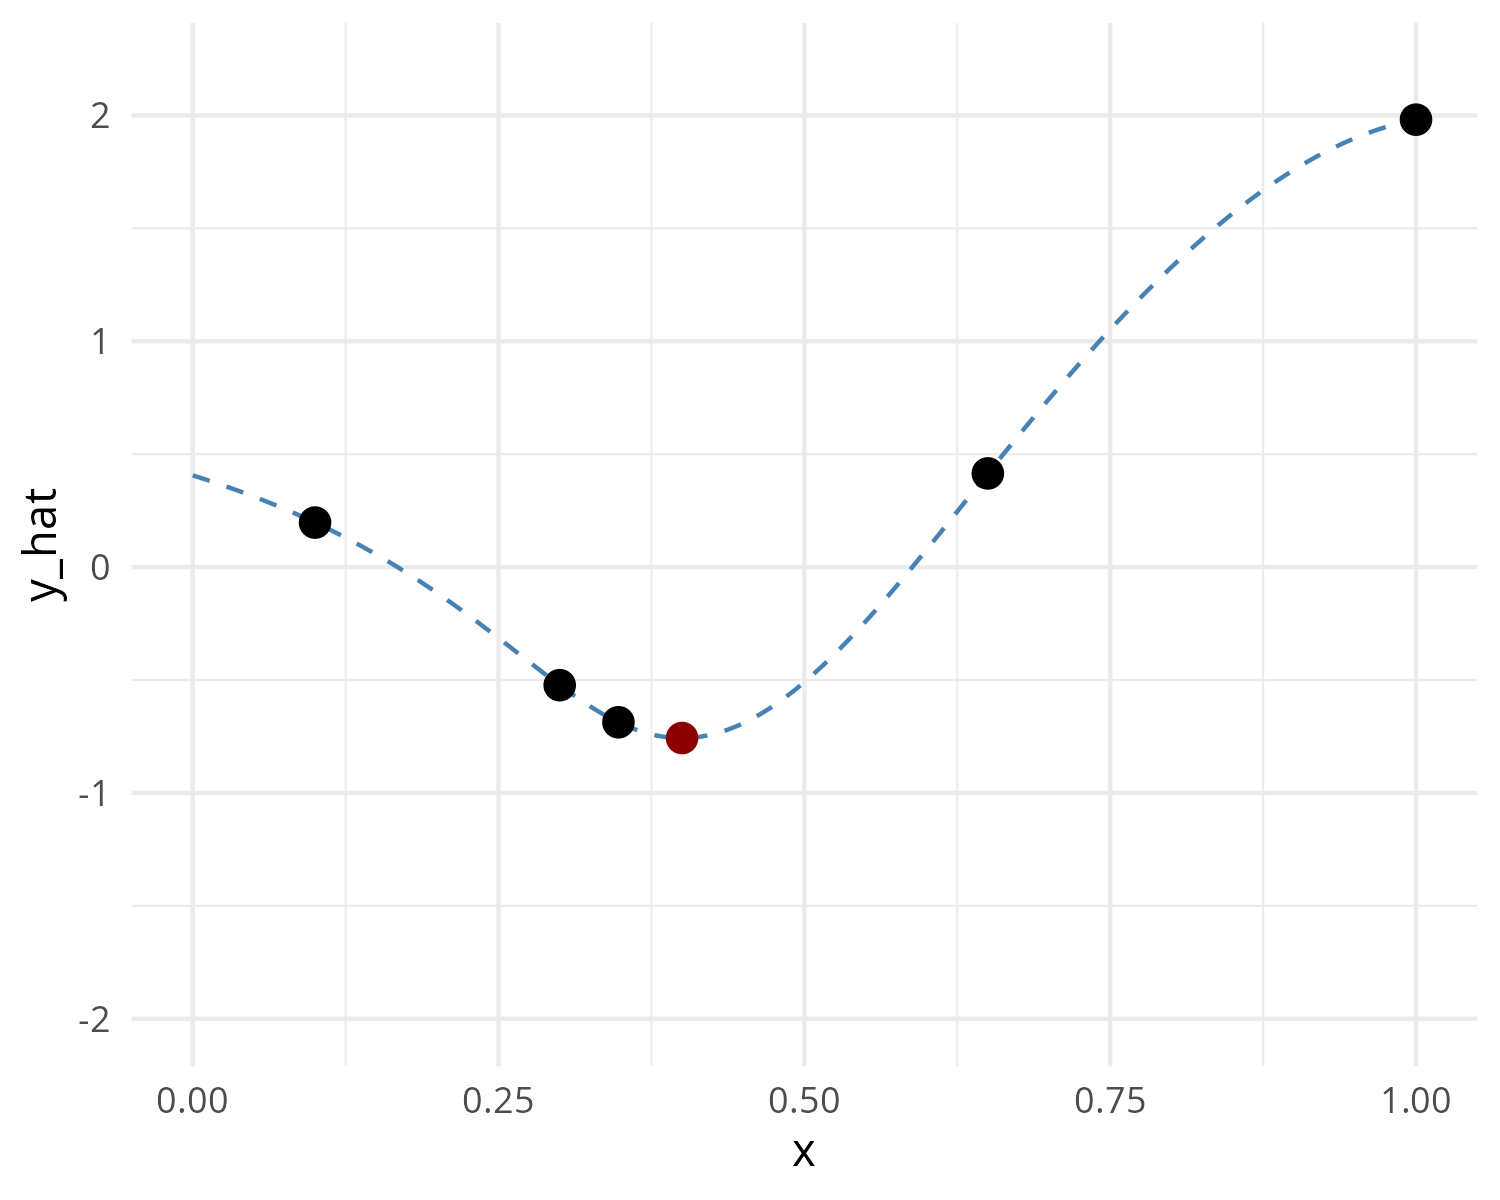
\includegraphics[width=.7\textwidth]{images/loop_6.png}
    \end{center}
\end{frame}

%----------------------------------------------------------------------

\begin{frame}{Surrogate Modeling}
    \ldots and evaluate that candidate.
    \vfill
    \begin{center}
        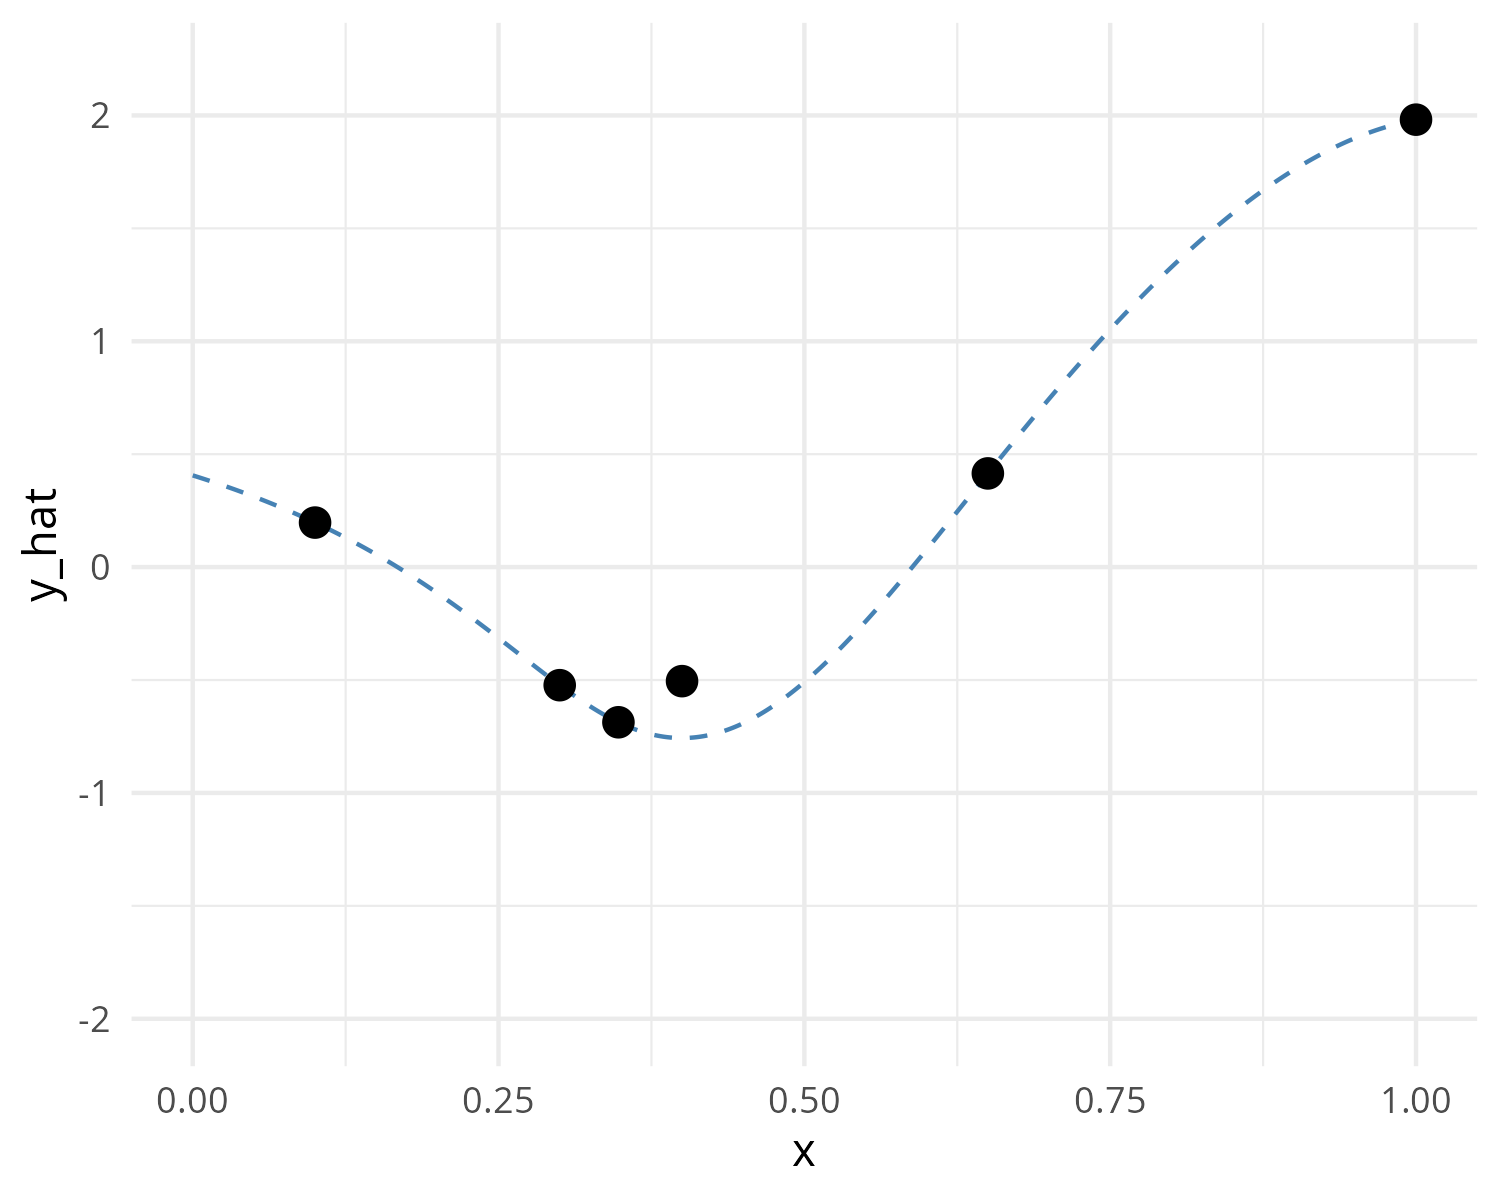
\includegraphics[width=.7\textwidth]{images/loop_7.png}
    \end{center}
\end{frame}

%----------------------------------------------------------------------

\begin{frame}{Surrogate Modeling}
    We repeat: (i) \textbf{fit} the model\ldots
    \vfill
    \begin{center}
        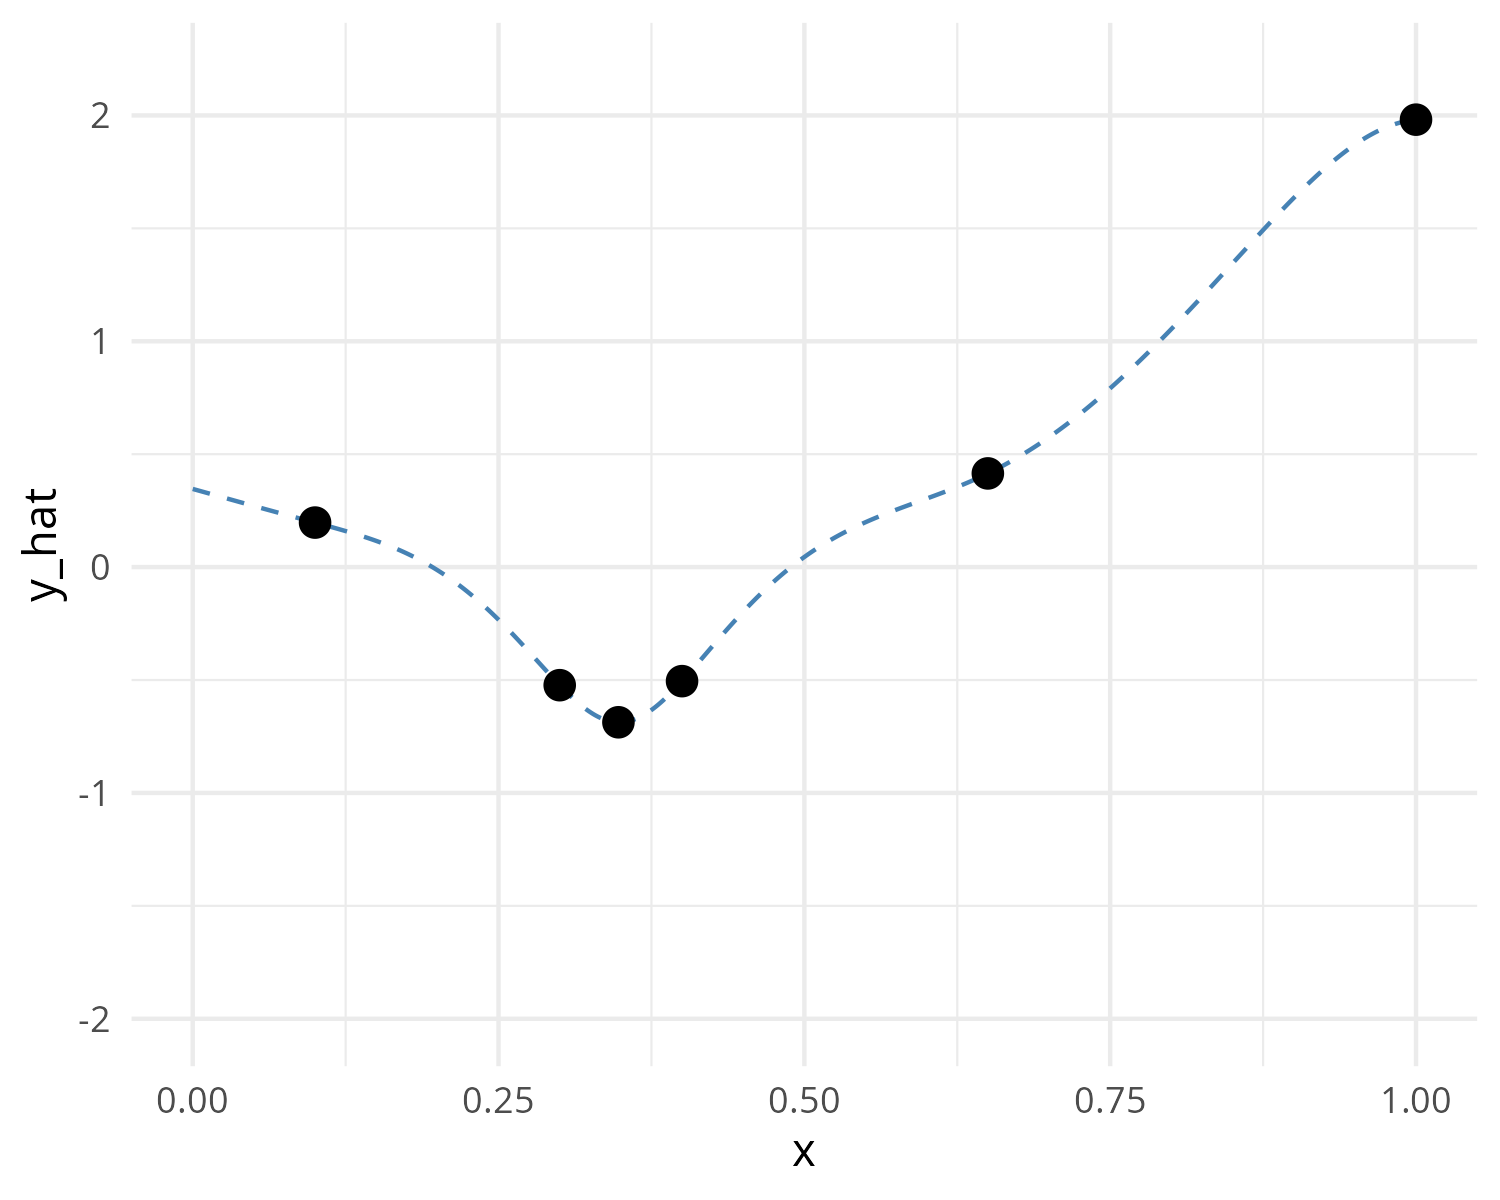
\includegraphics[width=.7\textwidth]{images/loop_8.png}
    \end{center}
\end{frame}

%----------------------------------------------------------------------

\begin{frame}{Surrogate Modeling}
    (ii) \textbf{propose} a new point\ldots
    \vfill
    \begin{center}
        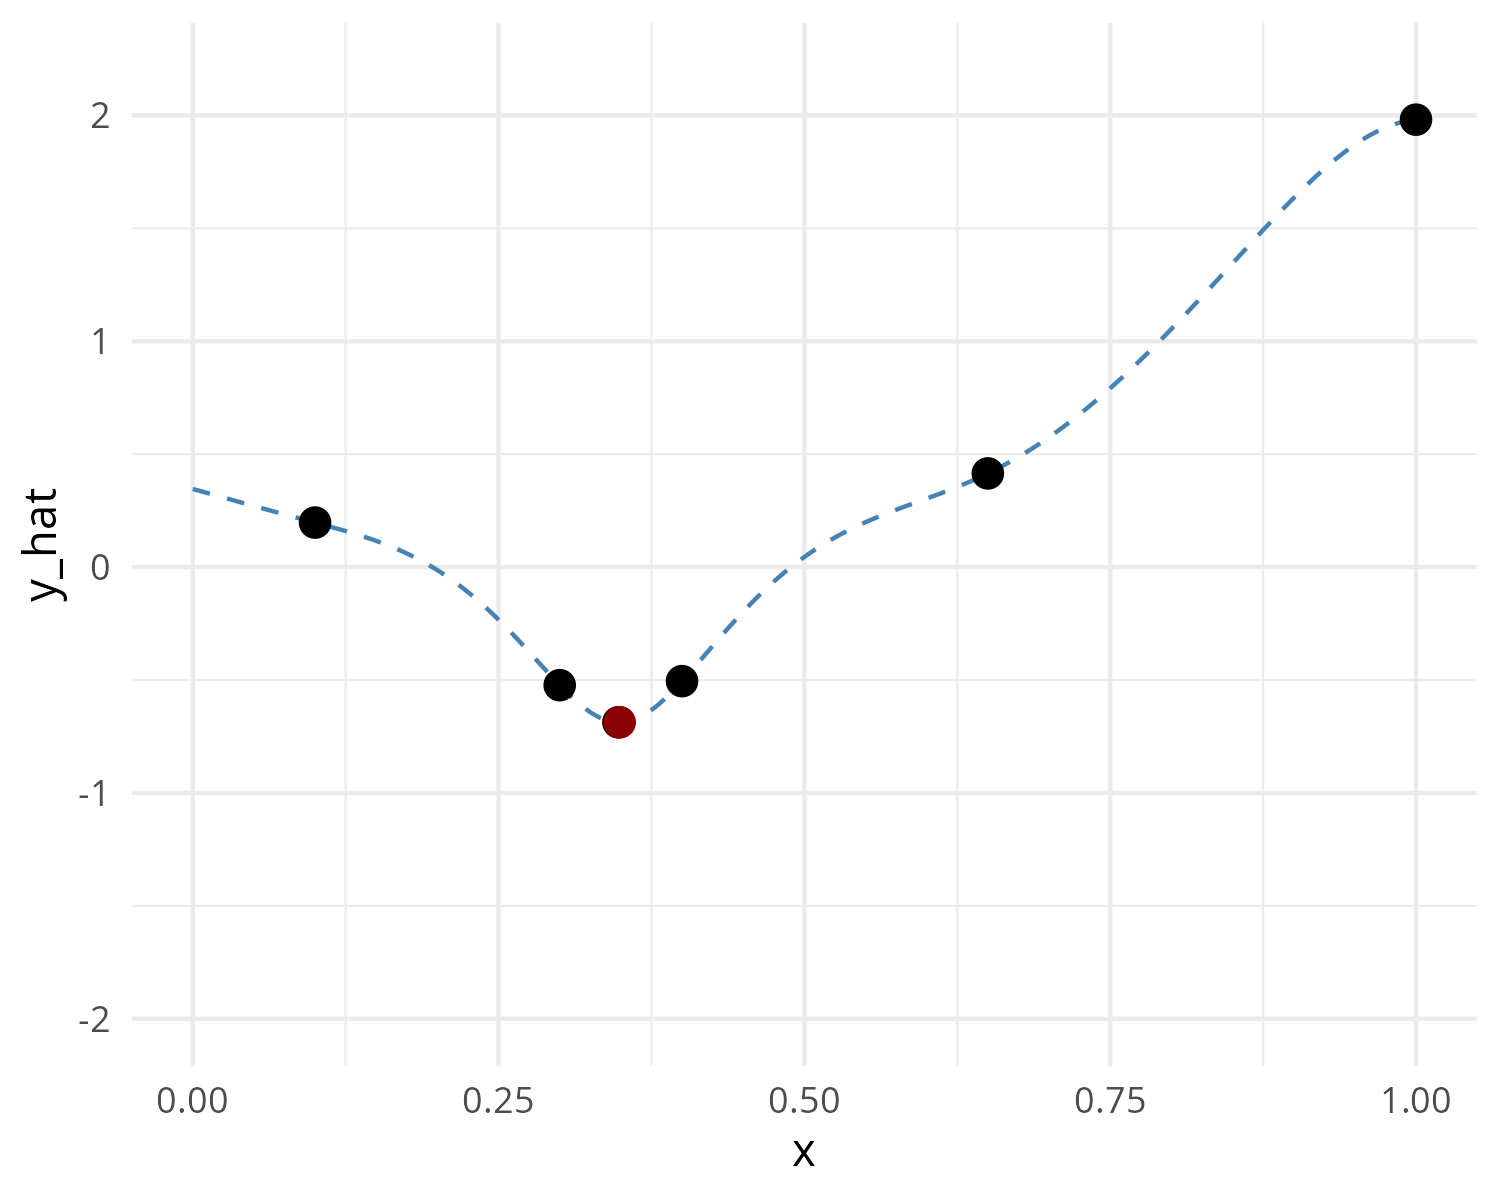
\includegraphics[width=.7\textwidth]{images/loop_9.png}
    \end{center}
\end{frame}

%----------------------------------------------------------------------

\begin{frame}{Surrogate Modeling}
    (iii) \textbf{evaluate} that point.
    \vfill
    \begin{center}
        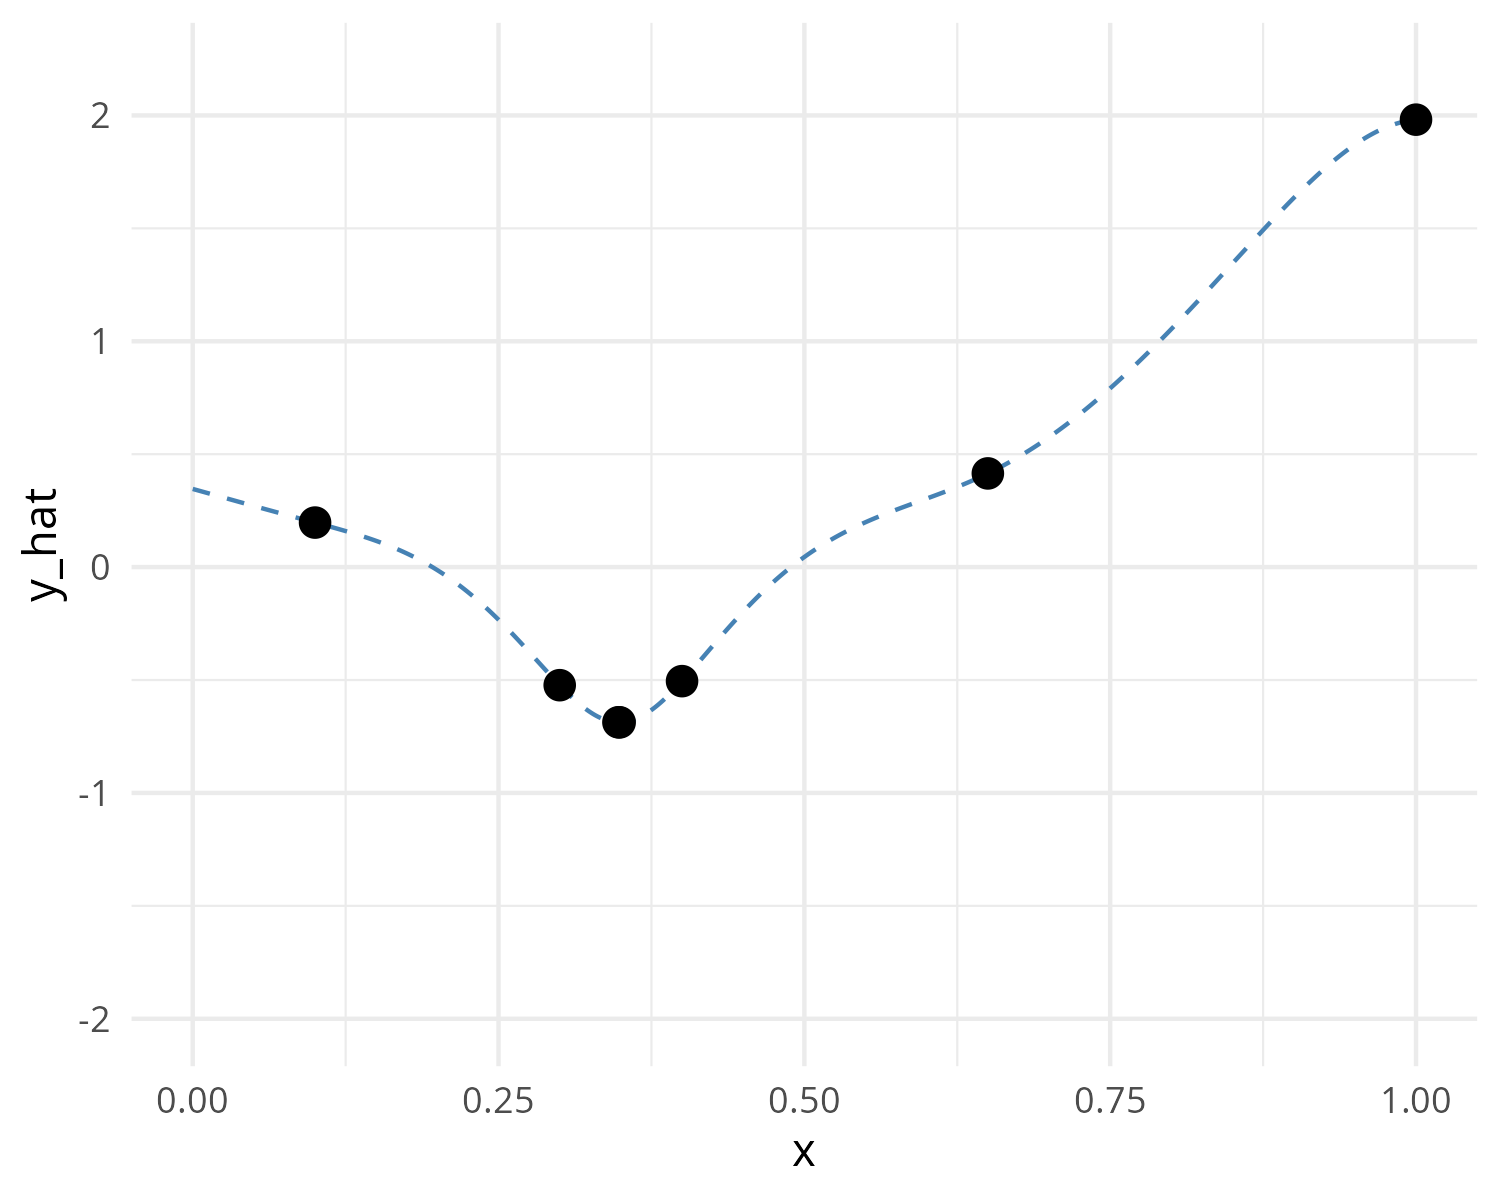
\includegraphics[width=.7\textwidth]{images/loop_10.png}
    \end{center}
    \begin{itemize}
        \item We observe that the algorithm converged.
    \end{itemize}
\end{frame}

%----------------------------------------------------------------------

\begin{frame}{Basic Loop}
    The basic loop of our sequential optimization procedure:
    \begin{enumerate}
        \item Fit surrogate model $\surro$ on previous evaluations $\Dts$
        \item Optimize the surrogate model $\surro$ to obtain a new point $\confI{t+1} := \argmin_{\conf \in \pcs} \surro(\conf)$
        \item Evaluate $\confI{t+1}$ and update data $\Dt[t+1] = \Dt \cup \{(\confI{t+1}, \cost(\confI{t+1}))\}$
    \end{enumerate}
\end{frame}

%----------------------------------------------------------------------

\begin{frame}{Exploration vs.\ Exploitation}
    We ran into a local minimum. We did not ``explore'' the most crucial areas and \textbf{missed} the global minimum.
    \vfill
    \begin{columns}
        \column{.5\textwidth}
        \begin{center}
            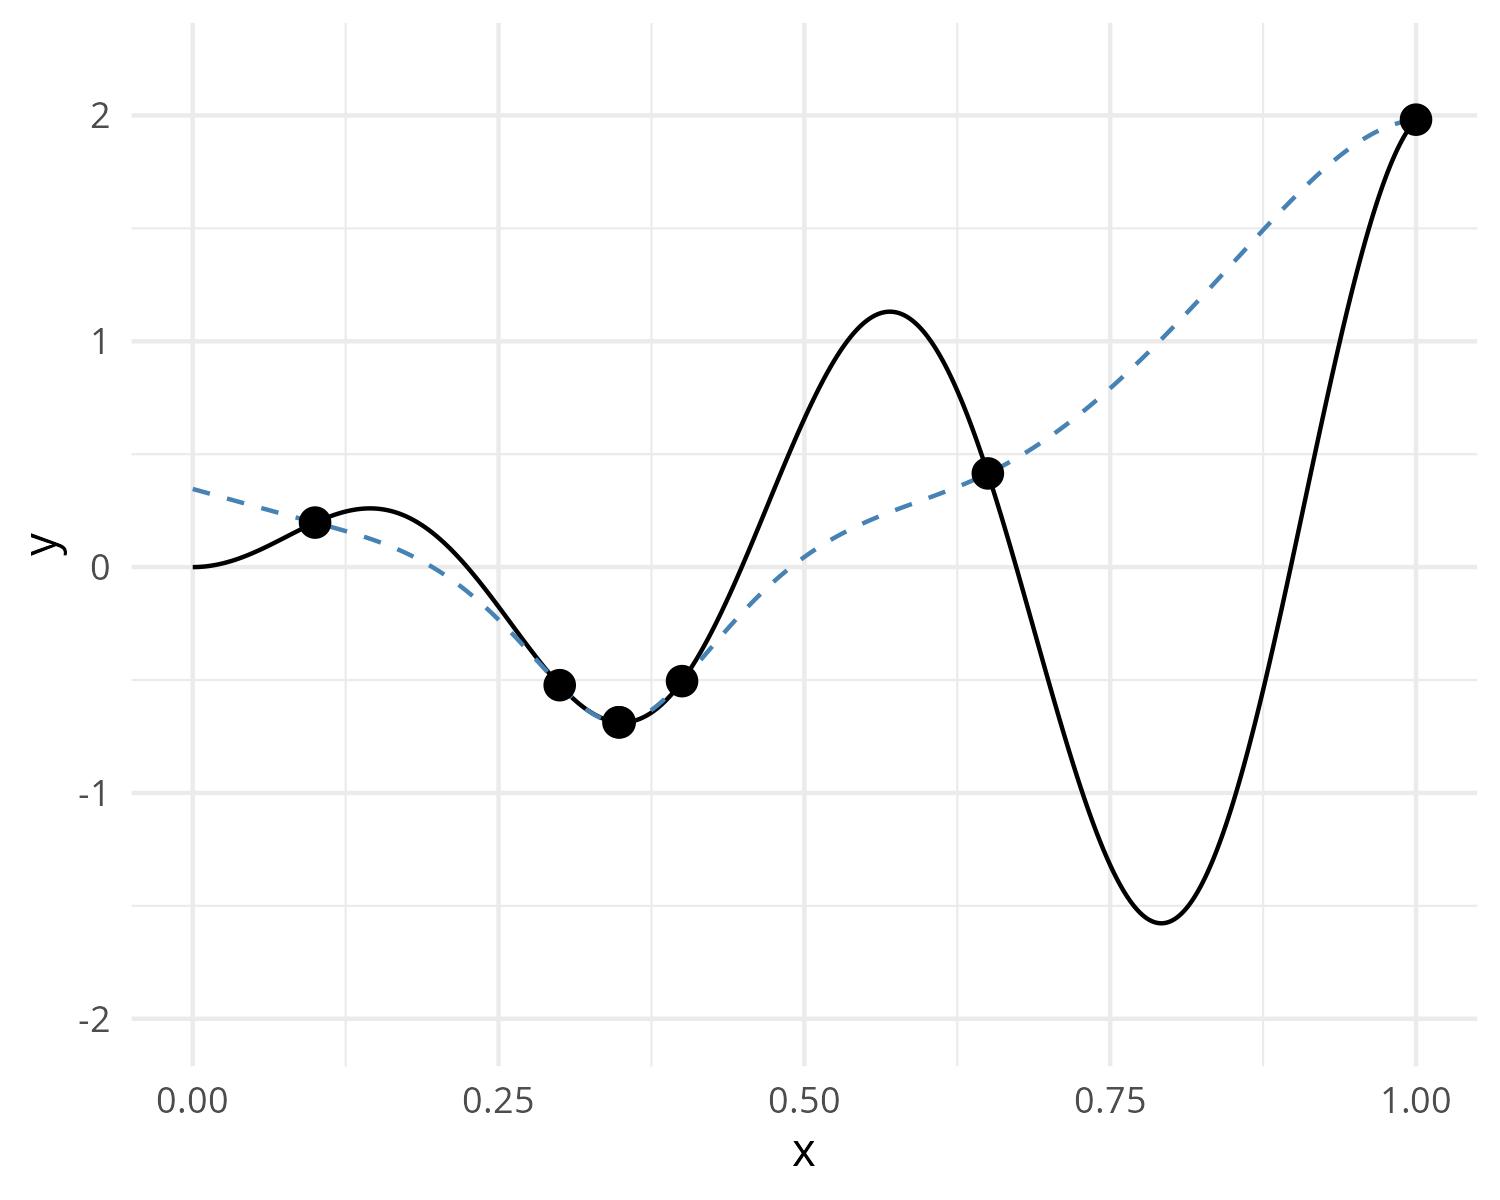
\includegraphics[width=\textwidth]{images/loop_11.png}
        \end{center}
        \column{.5\textwidth}
        \begin{itemize}
            \item Better ways to propose points based on our model exist, so-called \textbf{acquisition functions}
            \item Optimizing the surrogate directly corresponds to the raw / mean prediction as acquisition function
            \item Results in \textbf{high exploitation but low exploration}
        \end{itemize}
    \end{columns}
\end{frame}

%----------------------------------------------------------------------

\begin{frame}{Summary}
\begin{enumerate}
    \item BO starts with an initial design that covers the search space
    \item A surrogate model is fit to the evaluated points to approximate $\cost$
    \item The basic loop iterates: fit, propose, evaluate, update
    \item Using only the surrogate's mean prediction leads to strong exploitation but weak exploration
\end{enumerate}
\end{frame}

\end{document}
